\section{Multi-class Case}
We now consider the situation where there are $k > 2$ classes. 

We now define the analogous notion of `margin,' which will be important when we introduce the SVM model later.
\begin{definition}\label{margin_k_classes}
 Suppose that $k$ subsets of $\mathbb{R}^n$, $A_1,...,A_k$ are linearly separable by the matrix $W$ and vector $b$,
 and let $d$ be a metric on $\mathbb{R}^n$ as before. The margin of separation with respect to
 $d$ is given by
 \begin{equation}
  m(W,b; A_1,..., A_k) = \sup \{\epsilon:\text{$A^{\epsilon}_1,..., A^\epsilon_k$ are still linearly separated by $W$ and $b$}\}
 \end{equation}
where, as before, the $\epsilon$-enlargement of $A_i$ is given by
\begin{equation}
 A^\epsilon_i = \{y:\text{there is an $x\in A_i$ such that $\|x-y\| < \epsilon$}\}
\end{equation}
\end{definition}
This notion of margin measures how much we can perturb each data point without triggering a misclassification. This is 
quite a useful notion especially given the freedom to choose the metric $d$.

We close this section with a technical lemma relating compactness and the margin of separation, which can safely be skipped.
\begin{lemma}{\label{kclass_margin}}
 Suppose that the sets $A_1,...,A_k$ are separated by the matrix $W$ and vector $b$ and that $A_1,...,A_k$ are compact
 with respect to the topology induced by a metric $d$. Then
 \begin{equation}
  m(W,b; A_1,...,A_k) > 0
\end{equation}

\end{lemma}

\begin{proof}
	According to Lemma \ref{Interplation}, we only need to prove that for each $A_i$, there exists a positive number $\epsilon_i$ such that $A_i^{\epsilon_i}$ are still in $\Gamma_i(W,b)$. In fact, $\Gamma_i(W,b)$ is an open set, so $(\Gamma_i(W,b))^C$ and $A_i$ are two disjoint closed set. Thus we have
	\begin{equation}
	d_i = d(A_i,(\Gamma_i(W,b))^C) > 0
	\end{equation}
	We can take $\epsilon_i = d_i$. Actually, $d_i$ is the largest value that $\epsilon_i $ can take. And we have
	\begin{equation}
	m(W,b; A_1,...,A_k) =  \min_{i}~d_i > 0
	\end{equation}
\end{proof}


\subsection{k-class hard-margin Case}
In our examination of the $k$-class case, we first consider the situation where our data is linearly separable.

Assuming that our dataset is finite, and thus compact, we see that there exists an $\epsilon > 0$ such that
\begin{equation}
 w_i x+b_i \geq w_jx+b_j + \epsilon
\end{equation}
for all $x\in A_i$ and $j\neq i$, and a rescaling of $W$ and $b$ by $2\epsilon^{-1}$ means that we can assume without loss of 
generality that
\begin{equation}
 w_i x+b_i \geq w_jx+b_j + 2
\end{equation}
for all $x\in A_i$ and $j\neq i$. Or we can formulate it as
\begin{equation}\label{separation_constraint_k}
w_i x+b_i \geq \max_{j\neq i} (w_jx + b_j) + 2,~~\forall x\in A_i.
\end{equation}

%In order to simplify notation, we index our data points $x_1,...,x_N$ and introduce labels $y_1,...,y_N$, where
%\begin{equation}
% y_i = e_j~\text{if $x_i\in A_j$}
%\end{equation}
%i.e. $y_i$ is the standard basis vector corresponding to the class to which $x_i$ belongs. A clever and compact way of writing
%the linear separation constraint is now
%\begin{equation}\label{separation_constraint_k}
 %(y_i - e_j)\cdot (Wx_i+b) \geq \|y_i - e_j\|_1
%\end{equation}
%for all $i = 1,...,N$ and $j = 1,...,k$.

We note that the condition (\ref{separation_constraint_k}) is a collection of $Nk$ linear constraints on the matrix $W$ and
vector $b$. This means that we can determine whether our data is linearly separable by checking whether a given linear
program is feasible.

Of course, if our data is linearly separable, then we would like to find a matrix $W$ and vector $b$ which maximizes the
margin of separation as defined in Definition \ref{margin_k_classes}. To this end, we have the following lemma.
\begin{lemma}
 Assume that our data is separated by the matrix $W$ and vector $b$, and that (\ref{separation_constraint_k}) holds.
 Then the margin of separation is bounded below by
 \begin{equation}
  m(W,b;A_1,...,A_k)\geq \frac{1}{\max_{1\leq i\leq k}\|w_i\|}
 \end{equation}
 where $\|w_i\|$ is the dual norm of the $i$-th row of $w$.
\end{lemma}

\begin{proof}
	Use the notations in the proof of lemma \ref{kclass_margin}. Because $m(W,b, A_1,...,A_k) =  \min_{i}~d_i$, we only need to prove for each $i$, $d_i = d(A_i,\partial\Gamma_i(W,b)) \geq 1/\max_{1\leq i\leq k}\|w_i\|$.\\
	Take a point $x$ from $A_i$ and a point $y$ from $\partial\Gamma_i(W,b)$ arbitrarily. There exists $j\neq i$ such that
	$y \in H_{ij}$. So we have
	\begin{equation}
	\|x-y\| \geq d(x^i,H_{ij}) = \frac{|(w_i-w_j)x+(b_i-b_j)|}{\|w_i-w_j\|}\geq \frac{2}{\|w_i-w_j\|}\geq
	\frac{1}{\max_{1\leq i\leq k}\|w_i\|}.
	\end{equation}
    So we have
	\begin{equation}
	d_i = \inf_{y\in \partial\Gamma_i(W,b)} \|x-y\| \geq \frac{1}{\max_{1\leq i\leq k}\|w_i\|}.
	\end{equation}
	Above all, we can obtain
	\begin{equation}
	m_d(W,b;A_1,...,A_k) = \min_i~d_i \geq  \frac{1}{\max_{1\leq i\leq k}\|w_i\|}.
	\end{equation}
	
\end{proof}

This leads to the following convex optimization problem
\begin{align}{\label{kclass_hard_op}}
 \min_{W,~b~}~~&\max_{1\leq i\leq k}\|w_i\|\\
 s.t.~~&w_i x+b_i \geq \max_{j\neq i} (w_jx + b_j) + 2,~~\forall x\in A_i.
\end{align}
Naturally, we are interested in the relation between (\ref{kclass_hard_op}) for $k=2$ and $(\ref{2class_hard_op})$. It seems that we have done some relaxation in (\ref{kclass_hard_op}), but actually it is equivalent to $(\ref{2class_hard_op})$ in 2-class situations.
\begin{lemma}
The optimization problem (\ref{kclass_hard_op}) is equivalent to the problem $(\ref{2class_hard_op})$ when $k=2$.
\end{lemma} 
\begin{proof}
We'll set $k=2$ in the following statement. When $k=2$, the constraint (\ref{separation_constraint_k}) is equivalent to the constraint (\ref{separation_condition_2}), So we use (\ref{separation_condition_2}) to denote the constraint of both two problems. \\
We define three sets $\Omega,\Omega_1,\Omega_2$ as
\begin{gather}
\Omega = \{w~|~\exists b\in \mathbb{R},~\text{s.t.}~wx+b\geq 2, \forall x \in A_1~\text{and}~wx+b\leq -2, \forall x\in A_2\}.\\
\Omega_1 = \{(w_1,w_2)~|~w_1-w_2\in\Omega\}\\
\Omega_2 = \{(w_1,w_2)~|~w_1-w_2\in\Omega~\text{and}~w_1 = -w_2\}
\end{gather}
The constraint (\ref{separation_condition_2}) can be written as
\begin{equation}
(w_1,w_2)\in \Omega_1.
\end{equation}
Observing that $\Omega_2 \subset\Omega_1$, we'll show that for problem (\ref{kclass_hard_op}), nothing will change if we use the subset $\Omega_2$ to replace $\Omega_1$ in the constraint.\\
Take $(w_1,w_2)\in \Omega_1$ arbitrarily, and denote 
\[
\tilde{w}_1 = \frac{w_1-w_2}{2},~\tilde{w}_2 = -\frac{w_1-w_2}{2},
\]
then we have $(\tilde{w}_1,\tilde{w}_2)\in \Omega_2$ and
\begin{equation}
\max_{1\leq i\leq 2}\|\tilde{w}_i\| = \frac{1}{2} \|\tilde{w}_1-\tilde{w}_2\| = \frac{1}{2}\|w_1-w_2\| \leq \max_{1\leq i\leq 2}\|w_i\|.
\end{equation}
The inequalities above show that the element in $\Omega_1\backslash\Omega_2$ won't affect the solution of (\ref{kclass_hard_op}) at all. So we can use  $\Omega_2$ to replace $\Omega_1$ in problem (\ref{kclass_hard_op}), which means (\ref{kclass_hard_op}) is equivalent to 
\begin{equation}\label{proof_op1}
	\min_{(w_1,w_2)\in\Omega_2} \max_{1\leq i\leq 2}\|w_i\|.
\end{equation}
Also, easy to observe that the problem (\ref{separation_condition_2}) is equivalent to 
\begin{equation}\label{proof_op2}
\min_{(w_1,w_2)\in \Omega_2} \| w_1-w_2\|.
\end{equation}
For all $(w_1,w_2)\in \Omega_2$, we have
\begin{equation}
	\max_{1\leq i\leq 2}\|w_i\| = \frac{1}{2} \| w_1-w_2\|,
\end{equation}
which implies that the problem (\ref{proof_op1}) is equivalent to the problem (\ref{proof_op2}). \\
Consequently, the problem (\ref{2class_hard_op}) is equivalent to the problem (\ref{kclass_hard_op}) when $k=2$.
\end{proof}

\subsection{k-class soft-margin Case}
If the data is not max-mat linearly separable, then we replace the hard constraint (\ref{separation_constraint_k})
by a penalty term. A common choice of penalty is the hinge or ReLU loss, which only penalizes those constraints which are
not satisfied and leads to an optimization problem of the form
\begin{equation}{\label{kclass_soft_op}}
 \min_{W,~b}\max_{1\leq i\leq k}\|w_i\| + C\displaystyle\sum_{i=1}^k\displaystyle\sum_{x\in A_i}\text{ReLU}\Big( \max_{j\neq i} (w_jx + b_j) + 2 - (w_ix+b_i)\Big)
\end{equation}
where $C$ is a parameter controlling how much the penalty term is weighted.

When $k =2$, denoting $w_1-w_2$ as $w$, $b_1-b_2$ as $b$, we can write the 2-class soft margin optimization as 
\begin{equation}{\label{2-class soft-margin optimization}}
\min_{w,b} \|w\| + C\sum_{i=1}^2 \sum_{x\in A_i} ReLU((-1)^i (wx+b)+2)
\end{equation}

\section{Optimizaiton Problem in SVM}
From the discussion above, we transformed the classification problem into some optimization problems. In this section, we'll use Lagrange duality to transform the primal  problem into dual problem.  That will provide convinience for introducing the kernel method in SVM.\\
We first take a look at the hard-margin case as a transition to the soft-margin case.  Trivially, the problem (\ref{kclass_hard_op}) is equivalent to the following problem:
\begin{equation}
\begin{aligned}
\min_{W,~b} ~~& \max_{1\leq i\leq k}\|w_i\|,\\
s.t.               ~~& \|y_i - e_j\|_1 - (y_i - e_j)\cdot (Wx_i+b)\leq 0,~\forall i,j.\\
\end{aligned}
\end{equation}
For the introduction of inner product, here we take $\|\cdot\|=\|\cdot\|_2$, and use $\displaystyle\sum_{l=1}^k \|w_i\|_2^2$ to replace $\max_{1\leq i\leq k}\|w_i\|$. We can obtain a convex quadratic optimization problem for hard-margin case:
\begin{equation}{\label{kclass_hard_CQP}}
\begin{aligned}
\min_{W,~b} ~~& \frac{1}{2}\displaystyle\sum_{l=1}^k \|w_l\|_2^2,\\
s.t.               ~~& \|y_i - e_j\|_1 - (y_i - e_j)\cdot (Wx_i+b)\leq 0,~\forall i,j.\\
\end{aligned}
\end{equation}

Now let's turn to the soft-margin case. Similarly, we take $\|\cdot\|=\|\cdot\|_2$, and use $\displaystyle\sum_{l=1}^k \|w_i\|_2^2$ to replace $\max_{1\leq i\leq k}\|w_i\|$.

\begin{equation}{\label{kclass_soft_OP}}
\min_{W,~b}  \frac{1}{2}\displaystyle\sum_{i=1}^k \|w_i\|_2^2 + C\displaystyle\sum_{i=1}^N\displaystyle\sum_{j=1}^k\text{ReLU}\Big(\|y_i - e_j\|_1 - (y_i - e_j)\cdot (Wx_i+b)\Big)
\end{equation}

\begin{theorem}[Representer Theorem]
The solution of (\ref{kclass_soft_OP}) must belong to $span\{x_1,\cdots,x_N\}$, which means for each $i = 1,2,\cdots,k$, if $w_i^*$ is the optimal $w_i$ of (\ref{kclass_soft_OP}), then there must exist $\alpha_1^i,\cdots,\alpha_N^i\in \mathbb{R}$, such that  
\[
w_i^* = \sum_{j = 1}^N \alpha_j^i x_j.
\]
\end{theorem}

\begin{proof}
Denote $span\{x_1,\cdots,x_N\}$ as $X$ and the orthogonal projection operater on $X$ in $\mathbb{R}^n$ as $P$. Denote the objective function as $L(w_1,\cdots,w_k,b)$.\\
In fact, for each $i = 1,\cdots,k$, we have
\begin{align}
\|w_i\|_2^2 = ~&\|Pw_i + (w_i-Pw_i)\|_2^2 = \|Pw_i\|_2^2+\|w_i-Pw_i\|_2^2\geq \|Pw_i\|_2^2,\\
w_ix+b_i &= (Pw_i) x + b_i,~~\forall x \in\{x_1,\cdots,x_N\}.
\end{align}
So easy to observe that
\begin{align}
\sum_{i=1}^k &\|Pw_i\|_2^2\leq \sum_{i=1}^k \|w_i\|_2^2,\\
\max_{j\neq i} &((Pw_j)x + b_j) + 2 - ((Pw_i)x+b_i) = \max_{j\neq i} (w_jx + b_j) + 2 - (w_ix+b_i).
\end{align}
So we have
\begin{equation}
L(Pw_1,\cdots,Pw_k,b)\leq L(w_1,\cdots,w_k,b),
\end{equation}
which means the optimal $w_i$ for each $i\in\{1,\cdots,k\}$ must belong to $X$.
\end{proof}

We can obtain a similar convex quadratic optimization problem to (\ref{kclass_hard_CQP}) by introducing some slack variables $\xi$.

\begin{equation}{\label{kclass_soft_CQP}}
\begin{aligned}
\min_{W,b,\xi} ~~& \frac{1}{2}\displaystyle\sum_{j=1}^k \|w_j\|_2^2+C\displaystyle\sum_{i=1}^N\displaystyle\sum_{j=1}^k \xi_{ij},\\
s.t.               ~~& \|y_i - e_j\|_1 - (y_i - e_j)\cdot (Wx_i+b)-\xi_{ij} \leq 0,~\forall i,j.\\
                        & \xi_{ij} \geq 0,~\forall i,j.
\end{aligned}
\end{equation}

\begin{lemma}
The problem (\ref{kclass_soft_CQP}) is equivalent to the probelm (\ref{kclass_soft_OP}).
\end{lemma}
\begin{proof}
Denote the objetive functions as $f_1,f_2$:
\begin{equation}
\begin{split}
&f_1(W,b) = \frac{1}{2}\displaystyle\sum_{j=1}^k \|w_j\|_2^2 + C\displaystyle\sum_{i=1}^N\displaystyle\sum_{j=1}^k\text{ReLU}\Big(\|y_i - e_j\|_1 - (y_i - e_j)\cdot (Wx_i+b)\Big)\\
&f_2(W,b,\xi) = \frac{1}{2}\displaystyle\sum_{j=1}^k \|w_j\|_2^2+C\displaystyle\sum_{i=1}^N\displaystyle\sum_{j=1}^k \xi_{ij}.
\end{split}
\end{equation}
Easy to observe that 
\begin{equation}
	f_2(W,b,\xi)\leq f_1(W,b),
\end{equation}
equality holds iff 
\begin{equation}
    \xi_{ij} = \text{ReLU}\Big(\|y_i - e_j\|_1 - (y_i - e_j)\cdot (Wx_i+b)\Big).
\end{equation}
\end{proof}


It's easy to observe that the Slater's condition holds in the problem (\ref{kclass_soft_CQP}). That means we can obtain the optimal points of problem (\ref{kclass_soft_CQP}) by solving its dual problem.\\
The Lagrangian function of (\ref{kclass_soft_CQP}) is
\begin{equation}
\begin{aligned}
	&L(W,b,\xi,\lambda,\mu) \\
	= &\frac{1}{2}\displaystyle\sum_{j=1}^k \|w_j\|_2^2+C\displaystyle\sum_{i=1}^N\displaystyle\sum_{j=1}^k \xi_{ij} + \displaystyle\sum_{i=1}^N\displaystyle\sum_{j=1}^k \lambda_{ij}\Big(\|y_i - e_j\|_1 - (y_i - e_j)\cdot (Wx_i+b)-\xi_{ij}\Big) - \displaystyle\sum_{i=1}^N\displaystyle\sum_{j=1}^k \mu_{ij} \xi_{ij}\\
	= &\frac{1}{2}\displaystyle\sum_{j=1}^k \|w_j\|_2^2 + \displaystyle\sum_{i=1}^N\displaystyle\sum_{j=1}^k (C-\lambda_{ij}-\mu_{ij})\xi_{ij} + \displaystyle\sum_{i=1}^N\displaystyle\sum_{j=1}^k \lambda_{ij}\Big(\|y_i - e_j\|_1 - (y_i - e_j)\cdot (Wx_i+b)\Big)\\
	= &\frac{1}{2}\displaystyle\sum_{j=1}^k \|w_j\|_2^2 + \displaystyle\sum_{i=1}^N\displaystyle\sum_{j=1}^k (C-\lambda_{ij}-\mu_{ij})\xi_{ij} + \displaystyle\sum_{i=1}^N\Big(\delta_i-t_i\cdot (Wx_i)-t_i\cdot b\Big)
\end{aligned}
\end{equation}
where $\delta_i = \sum_{j=1}^k\lambda_{ij}\|y_i - e_j\|_1$, $t_i = \sum_{j=1}^k\lambda_{ij}(y_i - e_j)$, and $\lambda_{ij},\mu_{ij}\geq 0$.\\
The dual problem of (\ref{kclass_soft_CQP}) is 
\begin{equation}{\label{dual_problem}}
\max_{\lambda,\mu\geq 0} \min_{W,b,\xi} L(W,b,\xi,\lambda,\mu). 
\end{equation}
According to KKT conditions, we have 
\begin{equation}
\begin{aligned}
\nabla_{W}L(W^*,b^*,\xi^*,\lambda,\mu) &= W_* - \displaystyle\sum_{i=1}^N t_ix_i^{T} = 0,\\
\nabla_{b}L(W^*,b^*,\xi^*,\lambda,\mu)  &= -\displaystyle\sum_{i=1}^N t_i = 0,\\
\nabla_{\xi_{ij}}L(W^*,b^*,\xi^*,\lambda,\mu)  &= C-\lambda_{ij}-\mu_{ij} = 0,~\forall i,j..
\end{aligned}
\end{equation}
Take the equations above into dual problem (\ref{dual_problem}), we have
\begin{equation}
\begin{aligned}
&\min_{W,b,\xi} L(W,b,\xi,\lambda,\mu) \\
= &L(W^*,b^*,\xi^*,\lambda,\mu)\\ 
= &\frac{1}{2} Tr\Big((\displaystyle\sum_{i=1}^N t_i x_i^T)(\displaystyle\sum_{l=1}^N x_l t_l^T)\Big) -\displaystyle\sum_{i=1}^N t_i\cdot\Big((\displaystyle\sum_{l=1}^N t_l x_l^T)x_i\Big)+ \displaystyle\sum_{i=1}^N \delta_i\\
= &-\frac{1}{2}\displaystyle\sum_{i=1}^N\sum_{l=1}^N (t_i\cdot t_l)(x_i\cdot x_l)+ \displaystyle\sum_{i=1}^N \delta_i\\
= &-\frac{1}{2}\displaystyle\sum_{i=1}^N\sum_{l=1}^N\Big(\displaystyle\sum_{j=1}^k\sum_{m=1}^k \lambda_{ij}\lambda_{lm}(y_i-e_j)\cdot(y_l-e_m)\Big)(x_i\cdot x_l)+ \displaystyle\sum_{i=1}^N\sum_{j=1}^k\lambda_{ij}\|y_i - e_j\|_1
\end{aligned}
\end{equation}
So our dual problem can be transformed into the following form:
\begin{equation}{\label{SVM_dual}}
\begin{aligned}
\min_{\lambda}&~~ -\frac{1}{2}\displaystyle\sum_{i=1}^N\sum_{l=1}^N\Big(\displaystyle\sum_{j=1}^k\sum_{m=1}^k \lambda_{ij}\lambda_{lm}(y_i-e_j)\cdot(y_l-e_m)\Big)(x_i\cdot x_l)+ \displaystyle\sum_{i=1}^N\sum_{j=1}^k\lambda_{ij}\|y_i - e_j\|_1,\\
s.t.&~~\displaystyle \sum_{i=1}^N\sum_{j=1}^k\lambda_{ij}(y_i - e_j) = 0,\\
     &~~0\leq \lambda_{ij}\leq C,~\forall i,j.
\end{aligned}
\end{equation}

\section{Kernel Methods}
We denote the input space as $X$. Recalling that in the beginning of this chapter, we mentioned that a common way of obtaining a nonlinear classification model is to set $\mathscr{H} = \{\bm{f}: \bm{f}(x) = W\bm{\phi}(x)+b\}$, where $\bm{\phi}$ is a feature mapping from $X$ to a feature space $\mathcal{H}$. In other words, we use two steps to obtain a nonlinear classification model. First, we map input space $X$ to a feature space $\mathcal{H}$. Second, use linear classifier to do classification on $\bm\phi(X)\subset \mathcal{H}$.\\
Notice that if we use SVM on feature space, the optimization problem (\ref{SVM_dual}) turns to be
\begin{equation}{\label{SVM_dual}}
\begin{aligned}
\min_{W,~b}&~~ -\frac{1}{2}\displaystyle\sum_{i=1}^N\sum_{l=1}^N\Big(\displaystyle\sum_{j=1}^k\sum_{m=1}^k \lambda_{ij}\lambda_{lm}(y_i-e_j)\cdot(y_l-e_m)\Big)\langle\bm\phi(x_i),\bm\phi(x_l)\rangle+ \displaystyle\sum_{i=1}^N\sum_{j=1}^k\lambda_{ij}\|y_i - e_j\|_1,\\
s.t.&~~\displaystyle \sum_{i=1}^N\sum_{j=1}^k\lambda_{ij}(y_i - e_j) = 0,\\
&~~0\leq \lambda_{ij}\leq C,~\forall i,j.
\end{aligned}
\end{equation}
An interesting thing is that we actually only need to use the inner product of feature space in computation. That inspires us to focus on the inner product in feature space instead of the feature mapping itself.  We regard the inner product in feature space as a binary function on $X\times X$ and define it as a kernel function. In other words, a kernel function is $k: X\times X \rightarrow \mathbb{R}$ which
\begin{equation}
k(x,x) = \langle\bm\phi(x),\bm\phi(x')\rangle.
\end{equation}

\begin{definition}
Let $X$ be a non-empty set. Then a function $k:X\times X \rightarrow\mathbb{K}$ is
called a \textbf{kernel} on $X$ if there exists a $\mathbb{K}$-Hilbert space $\mathcal{H}$ and a map $\bm{\phi}:X\rightarrow \mathcal{H}$ such that for all $x \in X$ we have
\begin{equation}
k(x,x) = \langle\bm\phi(x),\bm\phi(x')\rangle.
\end{equation}
We call $\bm{\phi}$ a feature map and $\mathcal{H}$ a feature space of k.
\end{definition}

\begin{lemma}
Let $X$ be a non-empty set and $f_n:X\times X \rightarrow \mathbb{K}, n\in \mathbb{N}$, be functions such that $(f_n(x))\in l_2$ for all $x\in X$. Then 
\begin{equation}
k(x,x'):= \sum_{n=1}^{\infty} f_n(x) \overline{f_n(x')},~x,x'\in X,
\end{equation}
defines a kernel on $X$.
\end{lemma}

\begin{definition}
A function $k:X\times X \rightarrow \mathbb{R}$ is called \textbf{positive definite} if for all $n\in \mathbb{N}, ~\alpha_1,\cdots,\alpha_n\in \mathbb{R}$ and all $x_1,\cdots,x_n \in X$, we have
\begin{equation}{\label{positive_definite_kernel}}
\displaystyle\sum_{i=1}^n\sum_{j=1}^n\alpha_i \alpha_j k(x_j,x_i)\geq 0.
\end{equation}
Furthermore, $k$ is said to be \textbf{strictly positive definite} if, for mutually distinct $x_1,\cdots,x_n \in X$, equality in (\ref{positive_definite_kernel}) only holds for $\alpha_1=\cdots=\alpha_n=0$. Finnaly, $k$ is called \textbf{symmetric} if $k(x,x')=k(x',x)$ for all $x,x' \in X$.
\end{definition}

\begin{theorem}
A function $k:X\times X \rightarrow \mathbb{R}$ is a kernel if and only if it is symmetric and postive definite.
\end{theorem}
\begin{proof}
It is trivial that a kernel is a symmetric and postive definite function. We will mainly show the reverse implication.\\
Assuming $k$ is a positive definite kernel defined on $X$, we'll proceed to construct a feature mapping $\bm\phi$ into a Hilbert space for which $k$ is the kernel. We'll suppose that $X$ is an infinite set in the following discussion.
\begin{enumerate}
	\item Define the feature mapping $\bm\phi$ and construct a vector space $H_{pre}$.\\
	We define
	$$\bm\phi:x\longmapsto k(\cdot,x)$$
	According to this mapping, we span the image set to a vector space
	$$H_{pre}=\Big\{\sum_{i=1}^{n}\alpha_{i}k(\cdot,x_{i}):n\in\mathbb{N},\ \bm x_{i}\in X,~\alpha_{i}\in\mathbf{R},~i=1,\cdots,N \Big\}$$
	\item Make $H_{pre}$ an inner product space by defining inner product on $H_{pre}$.\\
	We define a binary function "$<\cdot,\cdot>$" on $H_{pre}$: for any $f,g\in \bm F$
	$$ f(\cdot)=\sum_{i=1}^{n}\alpha_{i}k(\cdot,x_{i}) $$
	$$ g(\cdot)=\sum_{j=1}^{m}\beta_{i}k(\cdot,x_{j}) $$
	$$ <f,g>=\sum_{i=1}^{n}\sum_{j=1}^{m}\alpha_{i}\beta_{j}k(x'_{j},x_{i}) $$
	The bilinearity and symmetry are easy to prove. Because the function$k$ is positive definite, we have
	$$ <f,f>=\sum_{i,j=1}^{m}\alpha_{i}\alpha_{j}k(x_{i},x_{j}),\forall\ f\in H_{pre} $$\\
	Use the symetric and positive definite property of Gram matrix, we can prove the Cauchy-Schwarz inequality
	\begin{equation}
	<f,g>^2\leqslant<f,f><g,g>
	\end{equation}
	Notice that
	\begin{equation}\label{reproducing property}
	<f, k(\cdot,x)>=\sum_{i=1}^{m}\alpha_{i}k(x_{i},x)=f(x)
	\end{equation}
	Take $g(\cdot)=k(\cdot,x)$ into (45), we have
	$$ <f,k(\cdot,x)>^2=|f(x)|^2\leq <f,f>k(x,x) $$
	So $<f,f>=0$ implies $f(x)\equiv 0$.
	Above all, binary function "$\bm\cdot$" satisfies bilinearity, symmetry and positive definiteness which suffices to show that "$<\cdot,\cdot>$" is an inner product on $H_{pre}$. \\
	Now vector space $H_{pre}$ equipped with inner product "$<\cdot,\cdot>$" is an inner product space.
	\item Complete the inner product space $H_{pre}$, we can get a Hilbert space $H$.\\
	Let $H$ be a completion of $H_{pre}$ and $I:H_{pre} \rightarrow H$ be the corresponding isometric embedding. Then $H$ is a Hilbert space and we have
	$$
	<Ik(\cdot,x'),Ik(\cdot,x)>_H=<k(\cdot,x'),k(\cdot,x)>_{H_{pre}}=k(x,x')
	$$
	for all $x,x'\in X, i.e., x\mapsto Ik(\cdot,x), x\in X$, defines a feature map of $k$.
	This Hilbert space is called $\textbf{reproducing\ kernel\ Hilbert\ space\ (RKHS)}$ because it satisfies equation (\ref{reproducing property}) which is called \textbf{reproducing property}.
\end{enumerate}
\end{proof}

\section{Relationship between SVM and Logistic Regression}
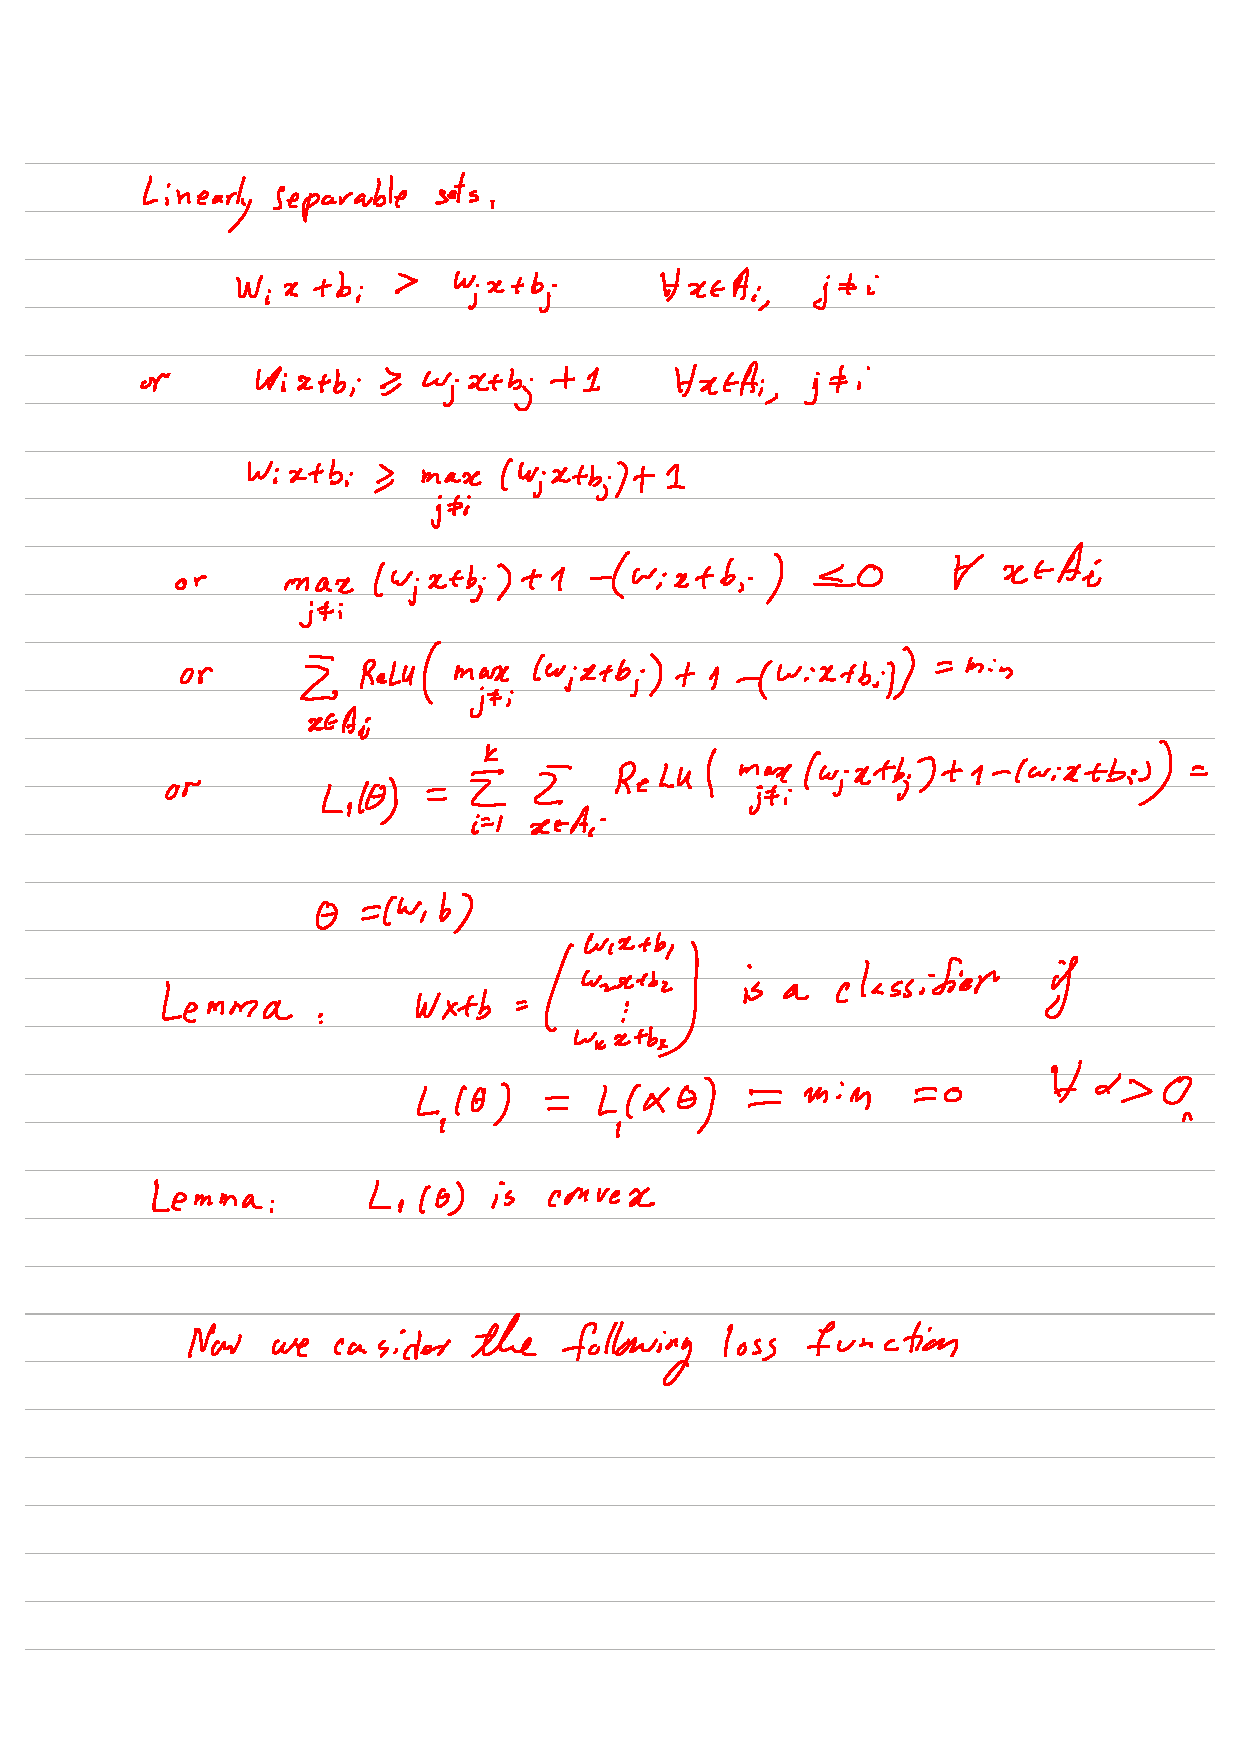
\includepdf[pages=-]{6DL/SVM-LR.pdf}
